\documentclass{exam}
\usepackage{graphicx} % Required for inserting images
\usepackage{amsmath}
\usepackage[left=3cm, right=3cm]{geometry}
\usepackage{multicol}
\usepackage{xcolor}
\usepackage{hyperref}

\printanswers % If you want to print answers
%\noprintanswers % If you don't want to print answers
% Specifies the way question are displayed:
\qformat{\textbf{Question\thequestion}\quad(\thepoints)\hfill}
\usepackage{color} % defines a new color
\definecolor{SolutionColor}{rgb}{0.8,0.9,1} % light blue
\shadedsolutions % defines the style of the solution environment
% \framedsolutions % defines the style of the solution environment
% Defines the title of the solution environment:
\renewcommand{\solutiontitle}{\noindent\textbf{Solution:}\par\noindent}

%\newcommand{\answer}[1]{\textcolor{blue}{#1}}
%\newcommand{\showanswers}{\let\answer\textcolor{blue}}
%\newcommand{\hideanswers}{\let\answer\phantom}

%\hideanswers

\title{Calculus aspects of the Greenhouse Effect}
%\author{Based on Primer by Philip Austin}
\date{}

\author{Raphael Kelly, Sven Bachmann, and Peter Harrington}

\begin{document}

\maketitle


\section*{Introduction -- Blackbody radiation}

\noindent Visible light is only a part of the spectrum of \emph{electromagnetic radiation} (EMR). EMR travels in waves and their frequency determines the energy they carry. The frequency $\nu$ and wavelength $\lambda$ are related by the equation \[\nu \lambda  = c\] where $c$ is the speed of light and it is a universal constant of nature. Within the visible spectrum, the wavelength of light is associated with a specific colour, as shown in Figure 1.

\noindent The unit of energy is the Joule $J$, the unit of frequency is $s^{-1}$ (also called the Herz $Hz$) and the unit of wavelength is $m$ (in particular, $\nu\lambda$ indeed has units of a velocity).

\begin{center}
    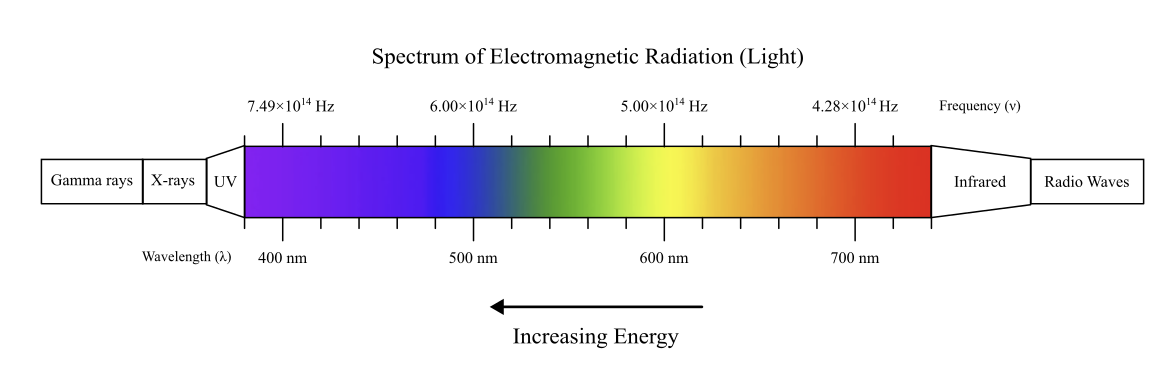
\includegraphics[scale=0.5]{spectrumofvisiblelight.png}
    \textbf{Figure 1.} The electromagnetic spectrum showing visible light as well as the classifications of light beyond the visible spectrum. Diagram not drawn to scale.
\end{center}

\noindent Matter in thermal equilibrium constantly absorbs and emits EMR. The physical processes underpinning these interactions depend on the temperature of the object and on the wavelength of the EMR. The intensity of the radiation at various wavelengths is given by the following \emph{Planck's law} of blackbody radiation\footnote{What this exactly means and a derivation of the formula would require much more physics, it is sufficient here to know that this blackbody is an idealization which is sufficiently good for our purpose.}:
$$B_T(\lambda) = \frac{2h c^2}{\lambda^5} \frac{1}{e^{\frac{h c}{\lambda k_B T}}-1}.$$
Specifically, the \emph{spectral radiance} $B_T(\lambda)$ is the rate of emitted radiation with wavelength $\lambda$ per unit surface area.

\begin{center}
    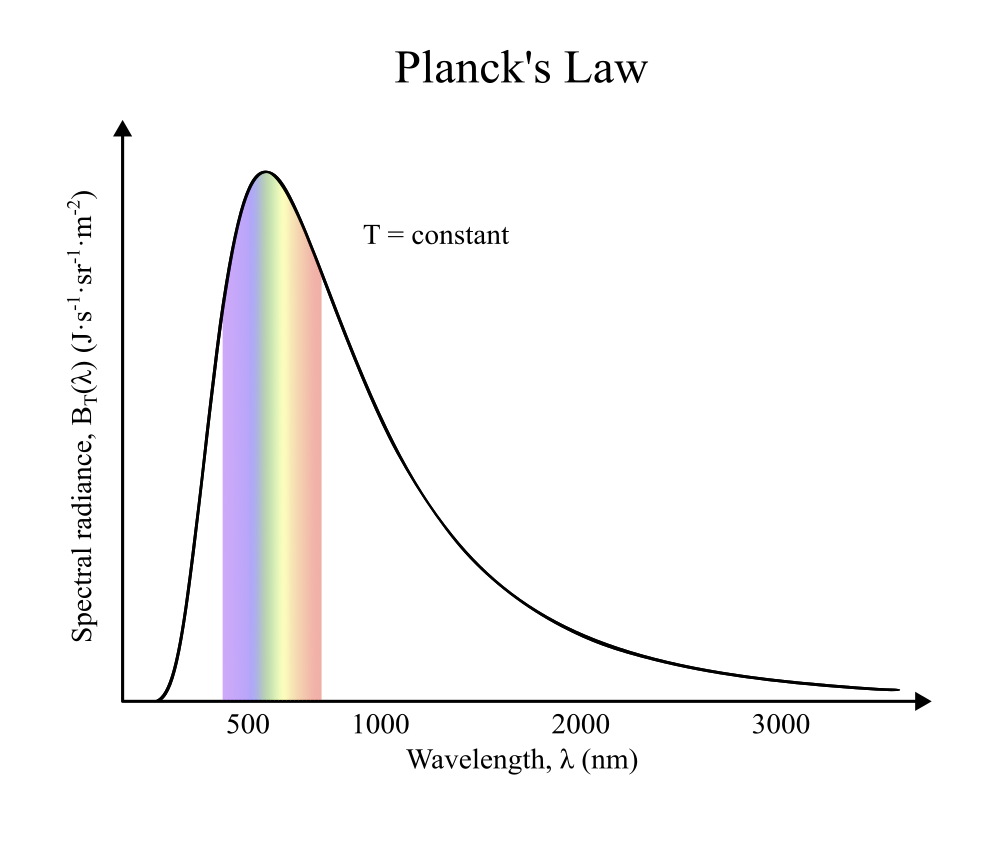
\includegraphics[scale=1.2]{planckslaw.png}
    
    \textbf{Figure 2.} The graph of $B_T(\lambda)$ for a fixed value of temperature $T = 5000K$.
\end{center}

Consider the table of variables and units below.

\begin{center}
\begin{tabular}{ l | l | l }
Symbol & Definition & (Value) Units \\
\hline \hline
$B_T$ & Spectral blackbody radiance & $J \cdot s^{-1} \cdot sr^{-1} \cdot 
 m^{-2} $ \\  
$\lambda$ & Wavelength & $m$ \\
$h$ & Planck's constant & $(6.63 \times 10^{-34}) J \cdot Hz^{-1}$ \\
$c$ & Speed of light & $(3.00 \times 10^{8}) m \cdot s^{-1}$ \\
$k_B$ & Boltzmann constant & $(1.38 \times 10^{-23}) J\cdot K^{-1}$
\end{tabular}
\end{center}

{\color{black} \noindent The units for $B_T$ are $J s^{-1} sr^{-1} m^{-2} $. The first part, $J s^{-1}$, denotes a rate of energy transfer (Joules per second). The second part, $sr^{-1} m^{-2}$, are (inverse) units of surface area. The symbol $sr$ stands for steradians which are a way to measure angles in three-dimensions. Just as $2\pi$ radians make up a circle, $4 \pi$ steradians make up a sphere.}

\newpage 

\section*{Part 1 -- Wien's displacement law (mainly Math 100 content)}
As can be observed in~Figure 2, Planck's law has one local maximum which is also its global maximum. Let $\lambda_{\mathrm{max}}$ be the critical point. In this question, we derive \emph{Wien's law}, which is the functional dependence of $\lambda_{\mathrm{max}}$ on the temperature $T$.

\begin{enumerate}
            \item Let the temperature $T$ be a fixed constant. Compute $\frac{d}{d\lambda}B_T(\lambda)$. 

     
            
            \item Consider the variable $$t=\frac{hc}{\lambda k_B T}.$$ Determine the equation characterizing the critical points of $B_T(\lambda)$ and write it in terms of the variable~$t$. Simplify the equation as much as possible but do not solve this equation.
  
            
            \item {\color{blue}Whether this is appropriate depends on how much of that is taught.} Show that there exists a solution $t_0\in(0,\infty)$ to the equation obtained in 2.

 

            \item {\color{blue}Same remark as above.} Show that there is exactly one solution $t_0\in(0,\infty)$ to the equation obtained in 2.

  
            
            \item Use the above to show that $B_T(\lambda)$ has a unique critical point $\lambda_{\mathrm{max}}$ and express it in terms of $t_0$.

   
            
            \item Conclude that Wien's displacement law holds: $$\lambda_{\mathrm{max}}=\frac{b}{T}$$ for some constant $b$ that is independent of the temperature. Express $b$ in terms of $t_0$ and the constants appearing the Planck's law.
  
            
            \item Show that $\lambda_{\mathrm{max}}$ is a global maximum of $B_T(\lambda)$ on the interval $(0, \infty)$.

          
            
            \item Using the information gathered so far, briefly explain why a flame changes colour from red to yellow to blue as it gets hotter.


\end{enumerate}

\section*{Part 2 - Stefan-Boltzmann's law (mainly Math 101 content)}
The total emitted energy per unit time and per unit surface area $I(T)$ is given by integrating over all wavelengths, namely $$I(T)= \int_0^\infty B_T(\lambda)d\lambda.$$ Stefan-Boltzmann's Law, which we shall derive here, is the fact that $I(T)$ is proportional to the fourth power of temperature. This steep dependence plays an important role in the earth's energy balance.
\begin{enumerate}

        \item Recall that $\lambda \nu = c$. Show that
    
        $$
        I(T) = \int_0^\infty \tilde B_T(\nu)d \nu,\qquad \text{where}\qquad\tilde{B}_T(\nu)=\frac{2h \nu^3}{c^2} \frac{1}{e^{\frac{h \nu}{k_B T}}-1}.
        $$



        \item Determine  $$\lim_{\nu \to 0+}\tilde{B}_T(\nu).$$ 

 
        \item Determine  $$\lim_{\nu \to \infty}\tilde{B}_T(\nu).$$

        
\end{enumerate}

We now wish to understand the asymptotic behaviour of $\tilde{B}_T(\nu)$ near the boundaries of the integration domain.  For this we use the notation $f(x)\approx g(x)$ as $x \to a$ whenever
%
\begin{equation*}
\lim_{x\to a}\frac{f(x)}{g(x)} = 1.
\end{equation*}
%
\begin{enumerate}
\setcounter{enumi}{3}
        \item Explain why $$\tilde{B}_T(\nu) \approx \frac{2\nu^2k_BT}{c^2}\qquad\text{as}\qquad\nu\to 0^+,$$ using a Taylor series expansion of the exponential function.


        \item Show that $$\tilde{B}_T(\nu) \approx \frac{2h\nu^3}{c^2}e^{-\frac{h\nu}{k_B T}}\qquad\text{as}\qquad\nu\to\infty.$$


                
        \item Use the asymptotics above to argue that $\int_0^\infty \tilde B_T(\nu)d \nu$ is a convergent integral. \\ \textit{Hint: You can use that $x^3 e^{-x}$ is smaller that $C e^{-x/2}$ for a large enough constant $C$.}



        \item Show that $$I(T)= \sigma \cdot T^4$$ for some positive constant $\sigma$ that is independent of the temperature. \\ \textit{Hint: This is an exercise in changing variables in an integral. You do not need to compute any integral to solve this question.}

  

        \item In the previous question, you should have encountered the integral $$ \xi = \int_0^\infty \frac{u^3}{e^u-1}du .$$ Because the integrand decays exponentially fast to zero at $\infty$ (see Question~3), the numerical value of $\xi$ is quite close to the value of $\int_0^N \frac{u^3}{e^u-1}du$ for $N=100$. \\ Numerically estimate the value of $\xi$ using Simpson's method with $N=100$ and $\Delta u=0.1$. Retain 5 decimal places and use the value of $\lim_{u \to 0^+} \frac{u^3}{e^u-1}$ in place of $\frac{u^3}{e^u-1}$ evaluated at zero.

  
        \item Compute $\sqrt[4]{15 \xi}$ using your numerical approximation of $\xi$. What number do you recognize?
  
        
        \item Write a symbolic expression for $\xi$ using what you determined previously and show that $I(T)=\sigma T^4$. \textit{Note: By symbolic, we mean write $\xi$ as a fraction using only integers and numbers like $e$, $\pi$, etc. Do not use any decimals.}


    \end{enumerate}



\section*{Part 3 -- The greenhouse effect (application of Wien's law from Part 1)}
We are now ready to understand one of the key processes underlying the role of $CO_2$ in the \emph{greenhouse effect}.
Gas molecules in the atmosphere absorb the energy of EMR that travels through them, but not all wavelengths are absorbed equally. The specific wavelengths that a gas tends to absorb is based upon its chemical composition, and can be expressed as an absorbance graph, see Figure 3. A larger value for absorbance at a given wavelength means that a layer of $CO_2$ absorbs more EMR of that specific wavelength.
\begin{center}
        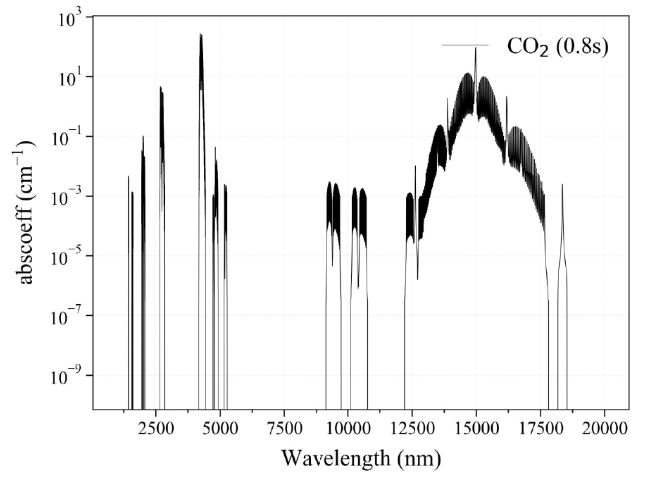
\includegraphics[scale=0.6]{image.png}
        
        \textbf{Figure 3.} The absorbance graph for $CO_2$, sourced from HITRAN online. This graph shows for example that $CO_2$ is essentially transparent to light around $7500nm$, but that it absorbs much of the light's energy around $15000nm$. The absorbance is negligible outside of the range of wavelengths displayed in the graph.
        % Source: \url{https://radis.readthedocs.io/en/latest/examples/hitran-spectra.html}
    \end{center}

    \noindent When a gas absorbs EMR, the incoming energy is transformed into molecular vibrations, resulting in an increase in the temperature of the gas.

\begin{enumerate}
        \item The sun is approximately a blackbody that emits EMR at its surface temperature of $5778K$. What wavelength of light is radiated the most abundantly by the sun? You can use that $b=2.9 \times 10^{-3} mK$.



        \item Does $CO_2$ in the atmosphere absorb much light from the sun?

 

        \item  As the radiation that has traversed the atmosphere reaches the earth, a fraction of it is immediately reflected while the rest is absorbed. The earth is in turn also an approximate blackbody and that emits radiation. What wavelength of light is radiated the most abundantly by the earth? You can use the temperature of the atmosphere at about $10km$, which is $223K$.



        \item Does $CO_2$ absorb much light from the Earth around $\lambda_{\mathrm{max}}$?



        \item Based on this information, discuss how the thermal emissions and selective absorbtions described above provide a mechanism for the greenhouse effect.

 
        
    \end{enumerate}

\end{document}